\documentclass{standalone}
\usepackage{tikz, xcolor}
\usetikzlibrary{shapes,arrows}

\begin{document}

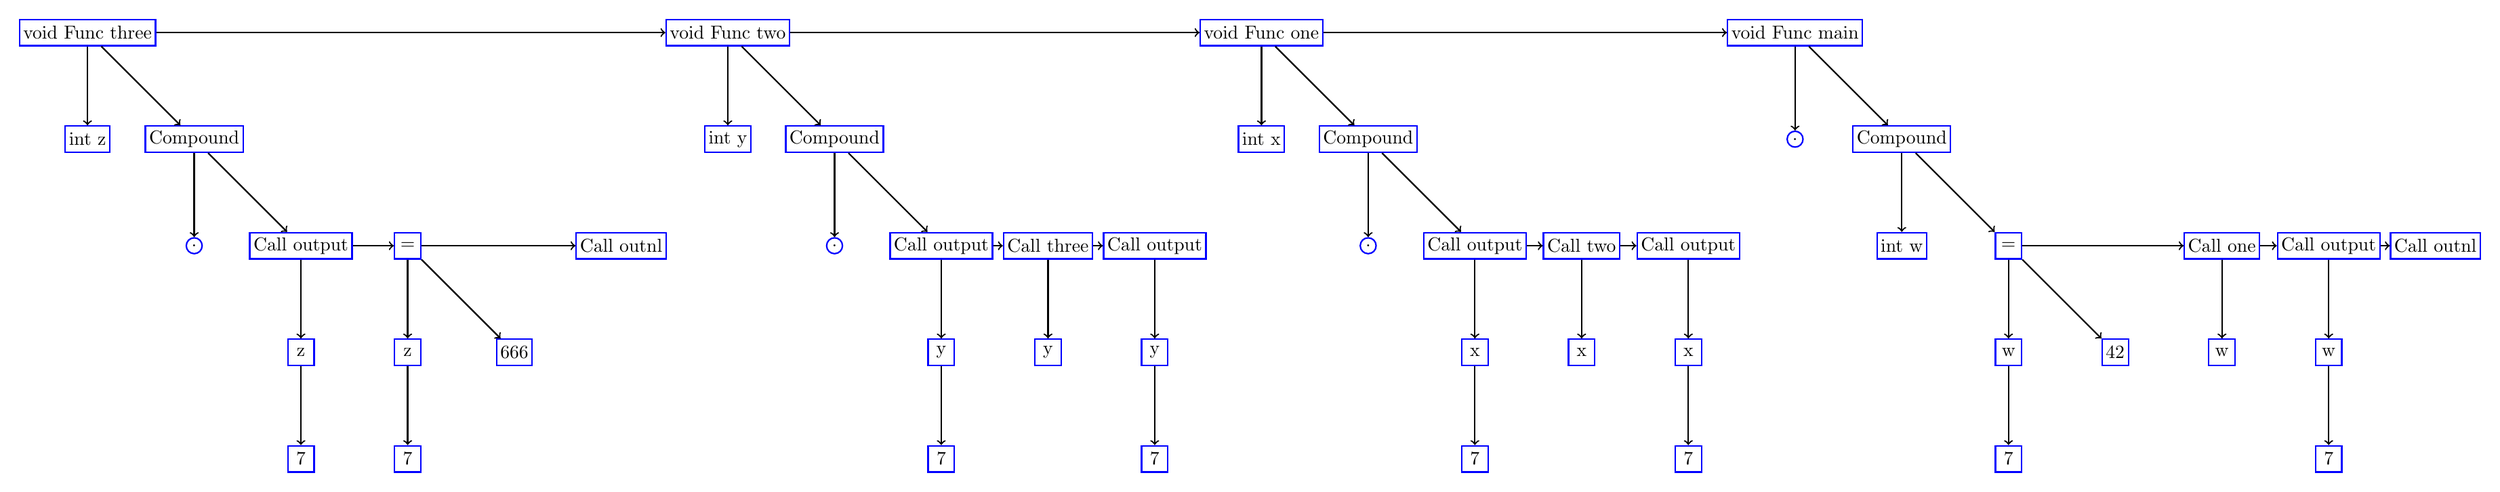
\begin{tikzpicture}[thick, scale=2.0]
\tikzstyle{vertexr}=[rectangle, draw=blue, thick, minimum size=14pt, inner sep=2pt]
\tikzstyle{vertexc}=[circle, draw=blue, thick, inner sep=2pt]
\tikzstyle{drawstyle}=[thick, ->]

\node[vertexr] (G0x0) at (0,0) {void Func three};
\node[vertexr] (G0x1) at (0,-1) {int z};
\draw[drawstyle] (G0x0) -- (G0x1);
\node[vertexr] (G1x1) at (1,-1) {Compound};
\node[vertexc] (G1x2) at (1,-2) {.};
\draw[drawstyle] (G1x1) -- (G1x2);
\node[vertexr] (G2x2) at (2,-2) {Call output};
\node[vertexr] (G2x3) at (2,-3) {z};
\node[vertexr] (G2x4) at (2,-4) {7};
\draw[drawstyle] (G2x3) -- (G2x4);
\draw[drawstyle] (G2x2) -- (G2x3);
\node[vertexr] (G3x2) at (3,-2) {=};
\node[vertexr] (G3x3) at (3,-3) {z};
\node[vertexr] (G3x4) at (3,-4) {7};
\draw[drawstyle] (G3x3) -- (G3x4);
\draw[drawstyle] (G3x2) -- (G3x3);
\node[vertexr] (G4x3) at (4,-3) {666};
\draw[drawstyle] (G3x2) -- (G4x3);
\node[vertexr] (G5x2) at (5,-2) {Call outnl};
\draw[drawstyle] (G3x2) -- (G5x2);
\draw[drawstyle] (G2x2) -- (G3x2);
\draw[drawstyle] (G1x1) -- (G2x2);
\draw[drawstyle] (G0x0) -- (G1x1);
\node[vertexr] (G6x0) at (6,0) {void Func two};
\node[vertexr] (G6x1) at (6,-1) {int y};
\draw[drawstyle] (G6x0) -- (G6x1);
\node[vertexr] (G7x1) at (7,-1) {Compound};
\node[vertexc] (G7x2) at (7,-2) {.};
\draw[drawstyle] (G7x1) -- (G7x2);
\node[vertexr] (G8x2) at (8,-2) {Call output};
\node[vertexr] (G8x3) at (8,-3) {y};
\node[vertexr] (G8x4) at (8,-4) {7};
\draw[drawstyle] (G8x3) -- (G8x4);
\draw[drawstyle] (G8x2) -- (G8x3);
\node[vertexr] (G9x2) at (9,-2) {Call three};
\node[vertexr] (G9x3) at (9,-3) {y};
\draw[drawstyle] (G9x2) -- (G9x3);
\node[vertexr] (G10x2) at (10,-2) {Call output};
\node[vertexr] (G10x3) at (10,-3) {y};
\node[vertexr] (G10x4) at (10,-4) {7};
\draw[drawstyle] (G10x3) -- (G10x4);
\draw[drawstyle] (G10x2) -- (G10x3);
\draw[drawstyle] (G9x2) -- (G10x2);
\draw[drawstyle] (G8x2) -- (G9x2);
\draw[drawstyle] (G7x1) -- (G8x2);
\draw[drawstyle] (G6x0) -- (G7x1);
\node[vertexr] (G11x0) at (11,0) {void Func one};
\node[vertexr] (G11x1) at (11,-1) {int x};
\draw[drawstyle] (G11x0) -- (G11x1);
\node[vertexr] (G12x1) at (12,-1) {Compound};
\node[vertexc] (G12x2) at (12,-2) {.};
\draw[drawstyle] (G12x1) -- (G12x2);
\node[vertexr] (G13x2) at (13,-2) {Call output};
\node[vertexr] (G13x3) at (13,-3) {x};
\node[vertexr] (G13x4) at (13,-4) {7};
\draw[drawstyle] (G13x3) -- (G13x4);
\draw[drawstyle] (G13x2) -- (G13x3);
\node[vertexr] (G14x2) at (14,-2) {Call two};
\node[vertexr] (G14x3) at (14,-3) {x};
\draw[drawstyle] (G14x2) -- (G14x3);
\node[vertexr] (G15x2) at (15,-2) {Call output};
\node[vertexr] (G15x3) at (15,-3) {x};
\node[vertexr] (G15x4) at (15,-4) {7};
\draw[drawstyle] (G15x3) -- (G15x4);
\draw[drawstyle] (G15x2) -- (G15x3);
\draw[drawstyle] (G14x2) -- (G15x2);
\draw[drawstyle] (G13x2) -- (G14x2);
\draw[drawstyle] (G12x1) -- (G13x2);
\draw[drawstyle] (G11x0) -- (G12x1);
\node[vertexr] (G16x0) at (16,0) {void Func main};
\node[vertexc] (G16x1) at (16,-1) {.};
\draw[drawstyle] (G16x0) -- (G16x1);
\node[vertexr] (G17x1) at (17,-1) {Compound};
\node[vertexr] (G17x2) at (17,-2) {int w};
\draw[drawstyle] (G17x1) -- (G17x2);
\node[vertexr] (G18x2) at (18,-2) {=};
\node[vertexr] (G18x3) at (18,-3) {w};
\node[vertexr] (G18x4) at (18,-4) {7};
\draw[drawstyle] (G18x3) -- (G18x4);
\draw[drawstyle] (G18x2) -- (G18x3);
\node[vertexr] (G19x3) at (19,-3) {42};
\draw[drawstyle] (G18x2) -- (G19x3);
\node[vertexr] (G20x2) at (20,-2) {Call one};
\node[vertexr] (G20x3) at (20,-3) {w};
\draw[drawstyle] (G20x2) -- (G20x3);
\node[vertexr] (G21x2) at (21,-2) {Call output};
\node[vertexr] (G21x3) at (21,-3) {w};
\node[vertexr] (G21x4) at (21,-4) {7};
\draw[drawstyle] (G21x3) -- (G21x4);
\draw[drawstyle] (G21x2) -- (G21x3);
\node[vertexr] (G22x2) at (22,-2) {Call outnl};
\draw[drawstyle] (G21x2) -- (G22x2);
\draw[drawstyle] (G20x2) -- (G21x2);
\draw[drawstyle] (G18x2) -- (G20x2);
\draw[drawstyle] (G17x1) -- (G18x2);
\draw[drawstyle] (G16x0) -- (G17x1);
\draw[drawstyle] (G11x0) -- (G16x0);
\draw[drawstyle] (G6x0) -- (G11x0);
\draw[drawstyle] (G0x0) -- (G6x0);
\end{tikzpicture}
\end{document}
Number of warnings: 0
Number of errors: 0
